\section{绪论}

\subsection{细胞大小的决定}

一般认为,细胞的大小取决于核糖体的活性,因为蛋白质的量由核糖体决定。最小的细胞是支原体。

从果蝇到哺乳动物,都应用一套几乎完全相同的信号网络来调控细胞大小。在哺乳动物中,这一网络的中心是一个名为mTOR(哺乳动物雷帕霉素靶蛋白\footnote{Mammalian target of rapamycin,因其能被雷帕霉素抑制得名。})的蛋白激酶。如果mTOR失活,细胞体积缩小。(\autoref{fig:mtor})

\begin{figure}[htbp]
	\centering
	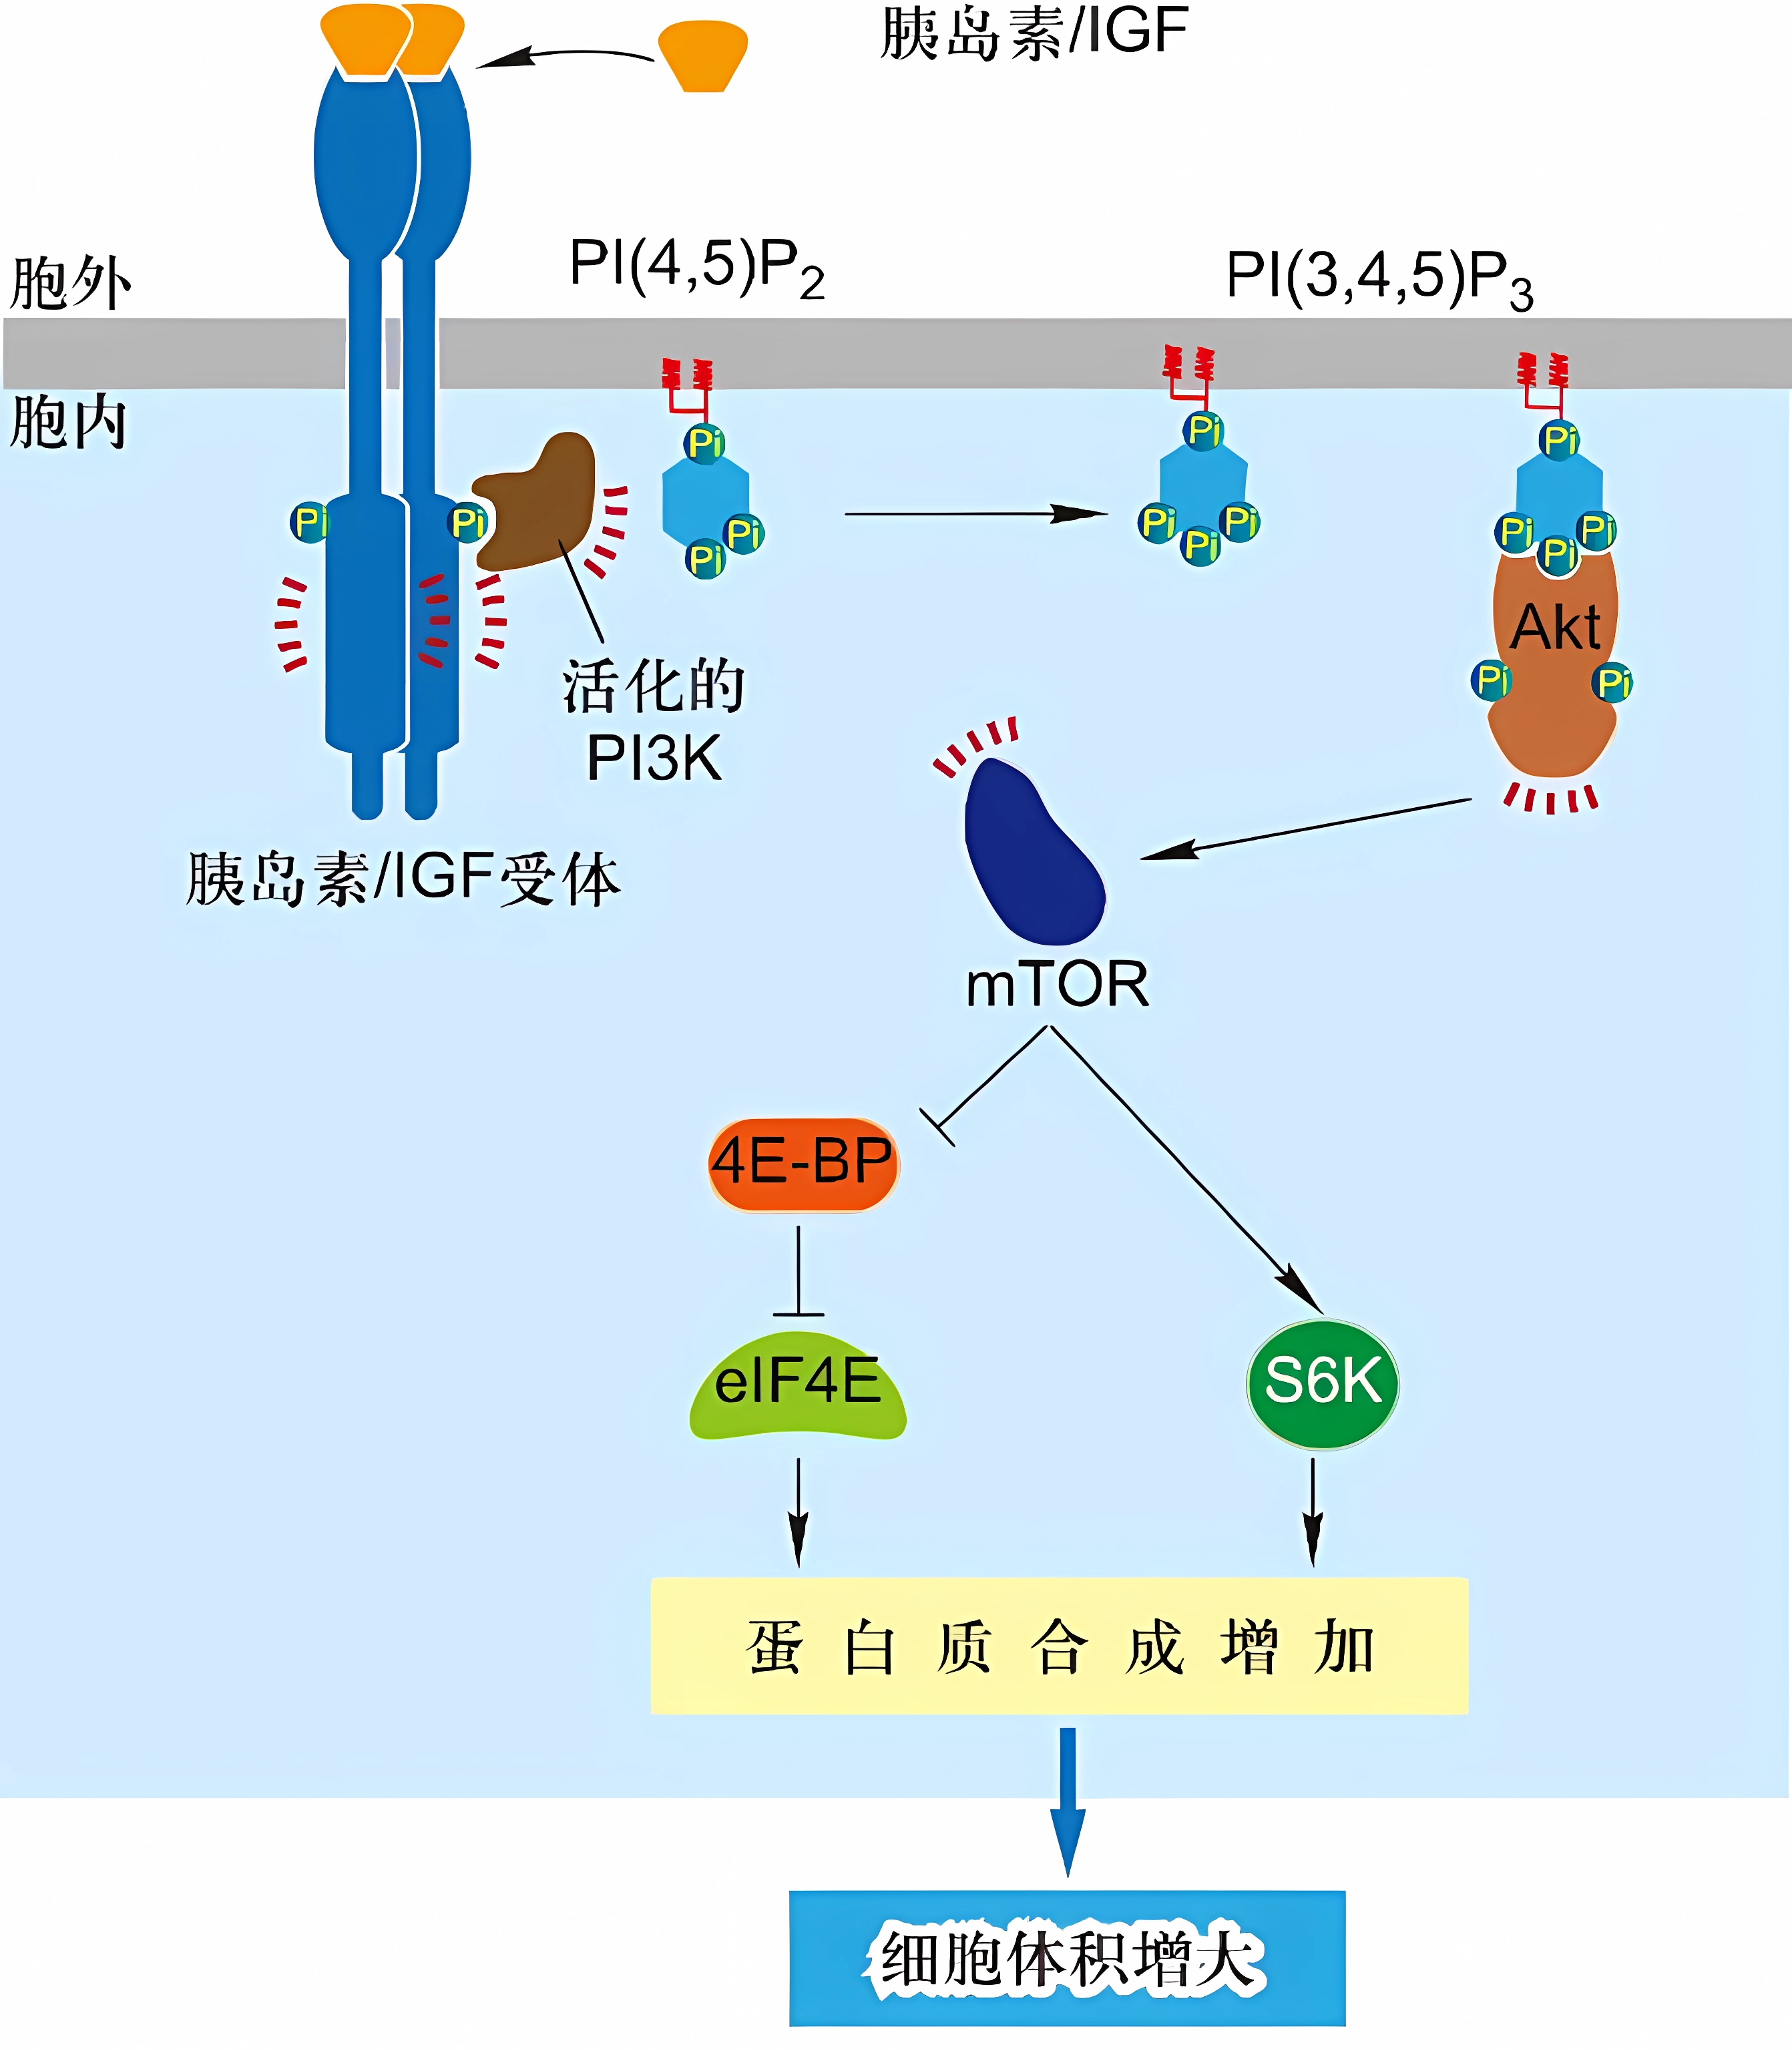
\includegraphics[width=0.5\textwidth]{Pics/mTOR}
	\caption{调控细胞大小的信号网络}
	\label{fig:mtor}
\end{figure}

\begin{figure}[htbp]
	\centering
	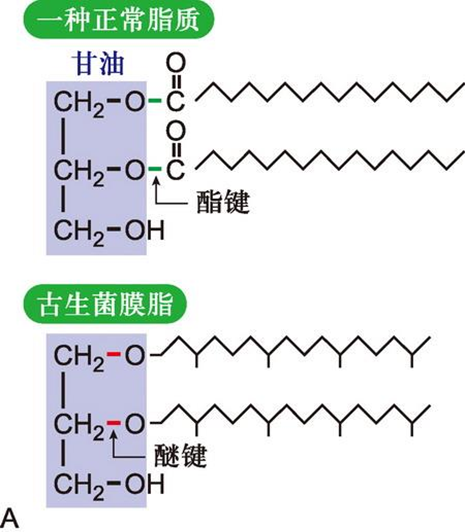
\includegraphics[width=.3\textwidth]{Pics/古细菌的细胞膜}
	\caption{古细菌膜脂的醚键}
	\label{fig:archaealMembraneLipidEtherBonds}
\end{figure}

细胞的大小还与其他因素有关,如植物细胞里液泡体积增大也会使细胞体积增大。

\subsection{古细菌(古核细胞)}

通过直系同源基因相似性比较,发现古细菌和真细菌在很早就分化了。很多古细菌都生活在极端环境中。



\begin{description}
	\item[细胞壁] 古细菌的细胞壁没有胞壁酸或肽聚糖,革兰氏染色呈阴性或阳性。
	\item[细胞质膜] 古细菌的膜脂是以醚键(\autoref{fig:archaealMembraneLipidEtherBonds})与甘油结合,膜脂中还含有鲨烯衍生物,是一种非极性脂质。
	\item[基因结构] 与细菌相似之处是:环状DNA、有操纵子、大部分无内含子、具多顺反子;与真核生物相似之处是:类似核小体的结构、部分基因有内含子、RNA聚合酶为复杂多聚体、翻译起始氨基酸是Met;
	\item[核糖体] 古核生物的核糖体与真核生物更接近,但多数古核生物核糖体是70S。抑制细菌核糖体的药物对古菌无效。
\end{description}

\section{细胞质膜}

\subsection{细胞质膜的结构}

\subsubsection{结构模型}

用锇酸固定细胞,由于锇酸与磷脂分子头部亲和力强,所以形成电镜中“暗-亮-暗”三层条带。(\autoref{fig:plasma_menb_em})

\begin{figure}[htbp]
	\centering
	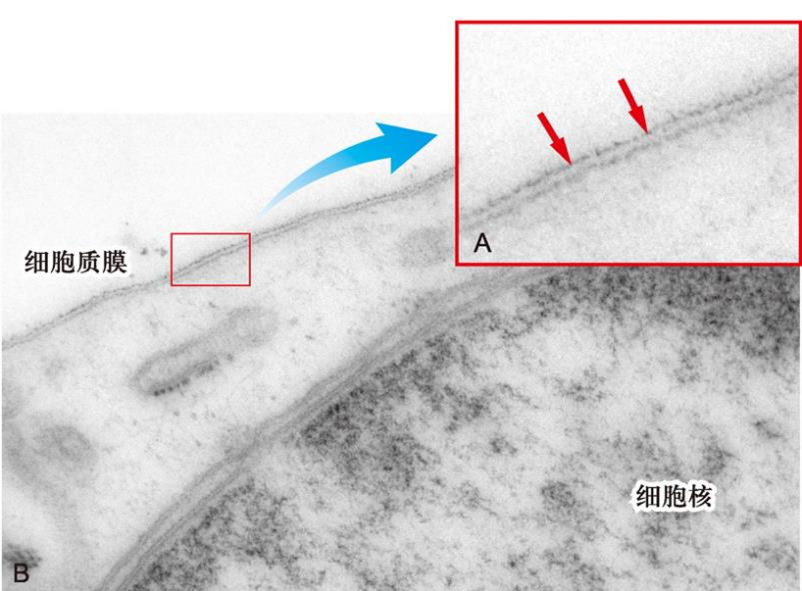
\includegraphics[width=0.5\linewidth]{Pics/电镜下的细胞质膜}
	\caption{电镜下的细胞质膜}
	\label{fig:plasma_menb_em}
\end{figure}

\paragraph{流动镶嵌模型}

在三明治模型、单位膜模型的基础上,Robertson提出了流动镶嵌模型。要点有:
\begin{itemize}
	\item 膜的流动性;
	\item 膜蛋白分布的不对称性。
\end{itemize}

\paragraph{脂筏模型}

脂筏模型是对膜流动性的新理解。脂筏模型认为:在脂双层上漂浮着小船一样的胆固醇、鞘磷脂的富集区域,载着可执行特定功能的膜蛋白。

\paragraph{目前对膜结构的认识}

\begin{itemize}
	\item 磷脂双分子层构成生物膜的基本结构。脂筏中存在有助于维持脂筏稳定的蛋白。
	\item 蛋白质镶嵌或结合在脂双层中或表面,赋予生物膜各自的功能。
	\item 膜中生物大分子的互相作用限制了膜的流动性,也形成了许多特殊结构(如耳蜗微绒毛)。
	\item 膜处在不断变化之中,保证了代谢活动正常进行。
\end{itemize}

\subsubsection{膜脂}

膜脂是生物膜的基本组成成分。

\paragraph{成分}





\section{物质跨膜运输}

\section{细胞质基质与内膜系统}

\section{蛋白质分选与膜泡运输}

\subsection{蛋白质分选}

\subsubsection{蛋白质分选的基本类型}

\subsubsection{蛋白质向线粒体和叶绿体的分选}

\begin{figure}[htbp]
	\centering
	\includegraphics[width=\linewidth]{Pics/核基因编码的线粒体蛋白转运}
	\caption{核基因编码的线粒体蛋白转运}
	\label{fig:tim_tom}
\end{figure}




\section{线粒体、叶绿体}



\section{细胞骨架}

细胞骨架,由粗到细包括:微管、中间丝、微丝。细胞骨架与数目众多的结合蛋白的相互作用,是细胞结构与功能相统一的分子基础。

\begin{figure}[h]
	\centering
	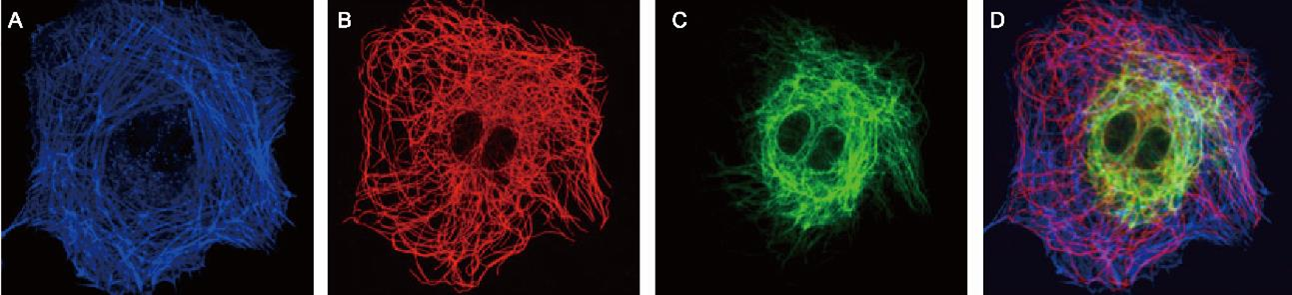
\includegraphics[width=0.9\linewidth]{Pics/cytoskeleton}
	\caption{免疫荧光染色示微丝(A)、微管(B)、中间丝(C)在体外培养的小鼠上皮细胞内的分布,以及叠加图(D)}
	\label{fig:cytoskeleton}
\end{figure}


\subsection{微丝}

微丝又称肌动蛋白丝,存在于所有真核细胞内。它的空间结构与功能取决于与之结合的微丝结合蛋白。在不同类型的细胞内,甚至是同一细胞的不同区域,不同的微丝结合蛋白赋予微丝不同的结构和功能。在三类细胞骨架中,微丝更接近细胞的边缘。(\autoref{fig:cytoskeleton})

以下活动有微丝的参与:细胞突起(微绒毛、伪足)、胞质分裂、吞噬作用、细胞迁移、肌球蛋白运动、细胞收缩、物质运输等。

\begin{figure}
	\centering
	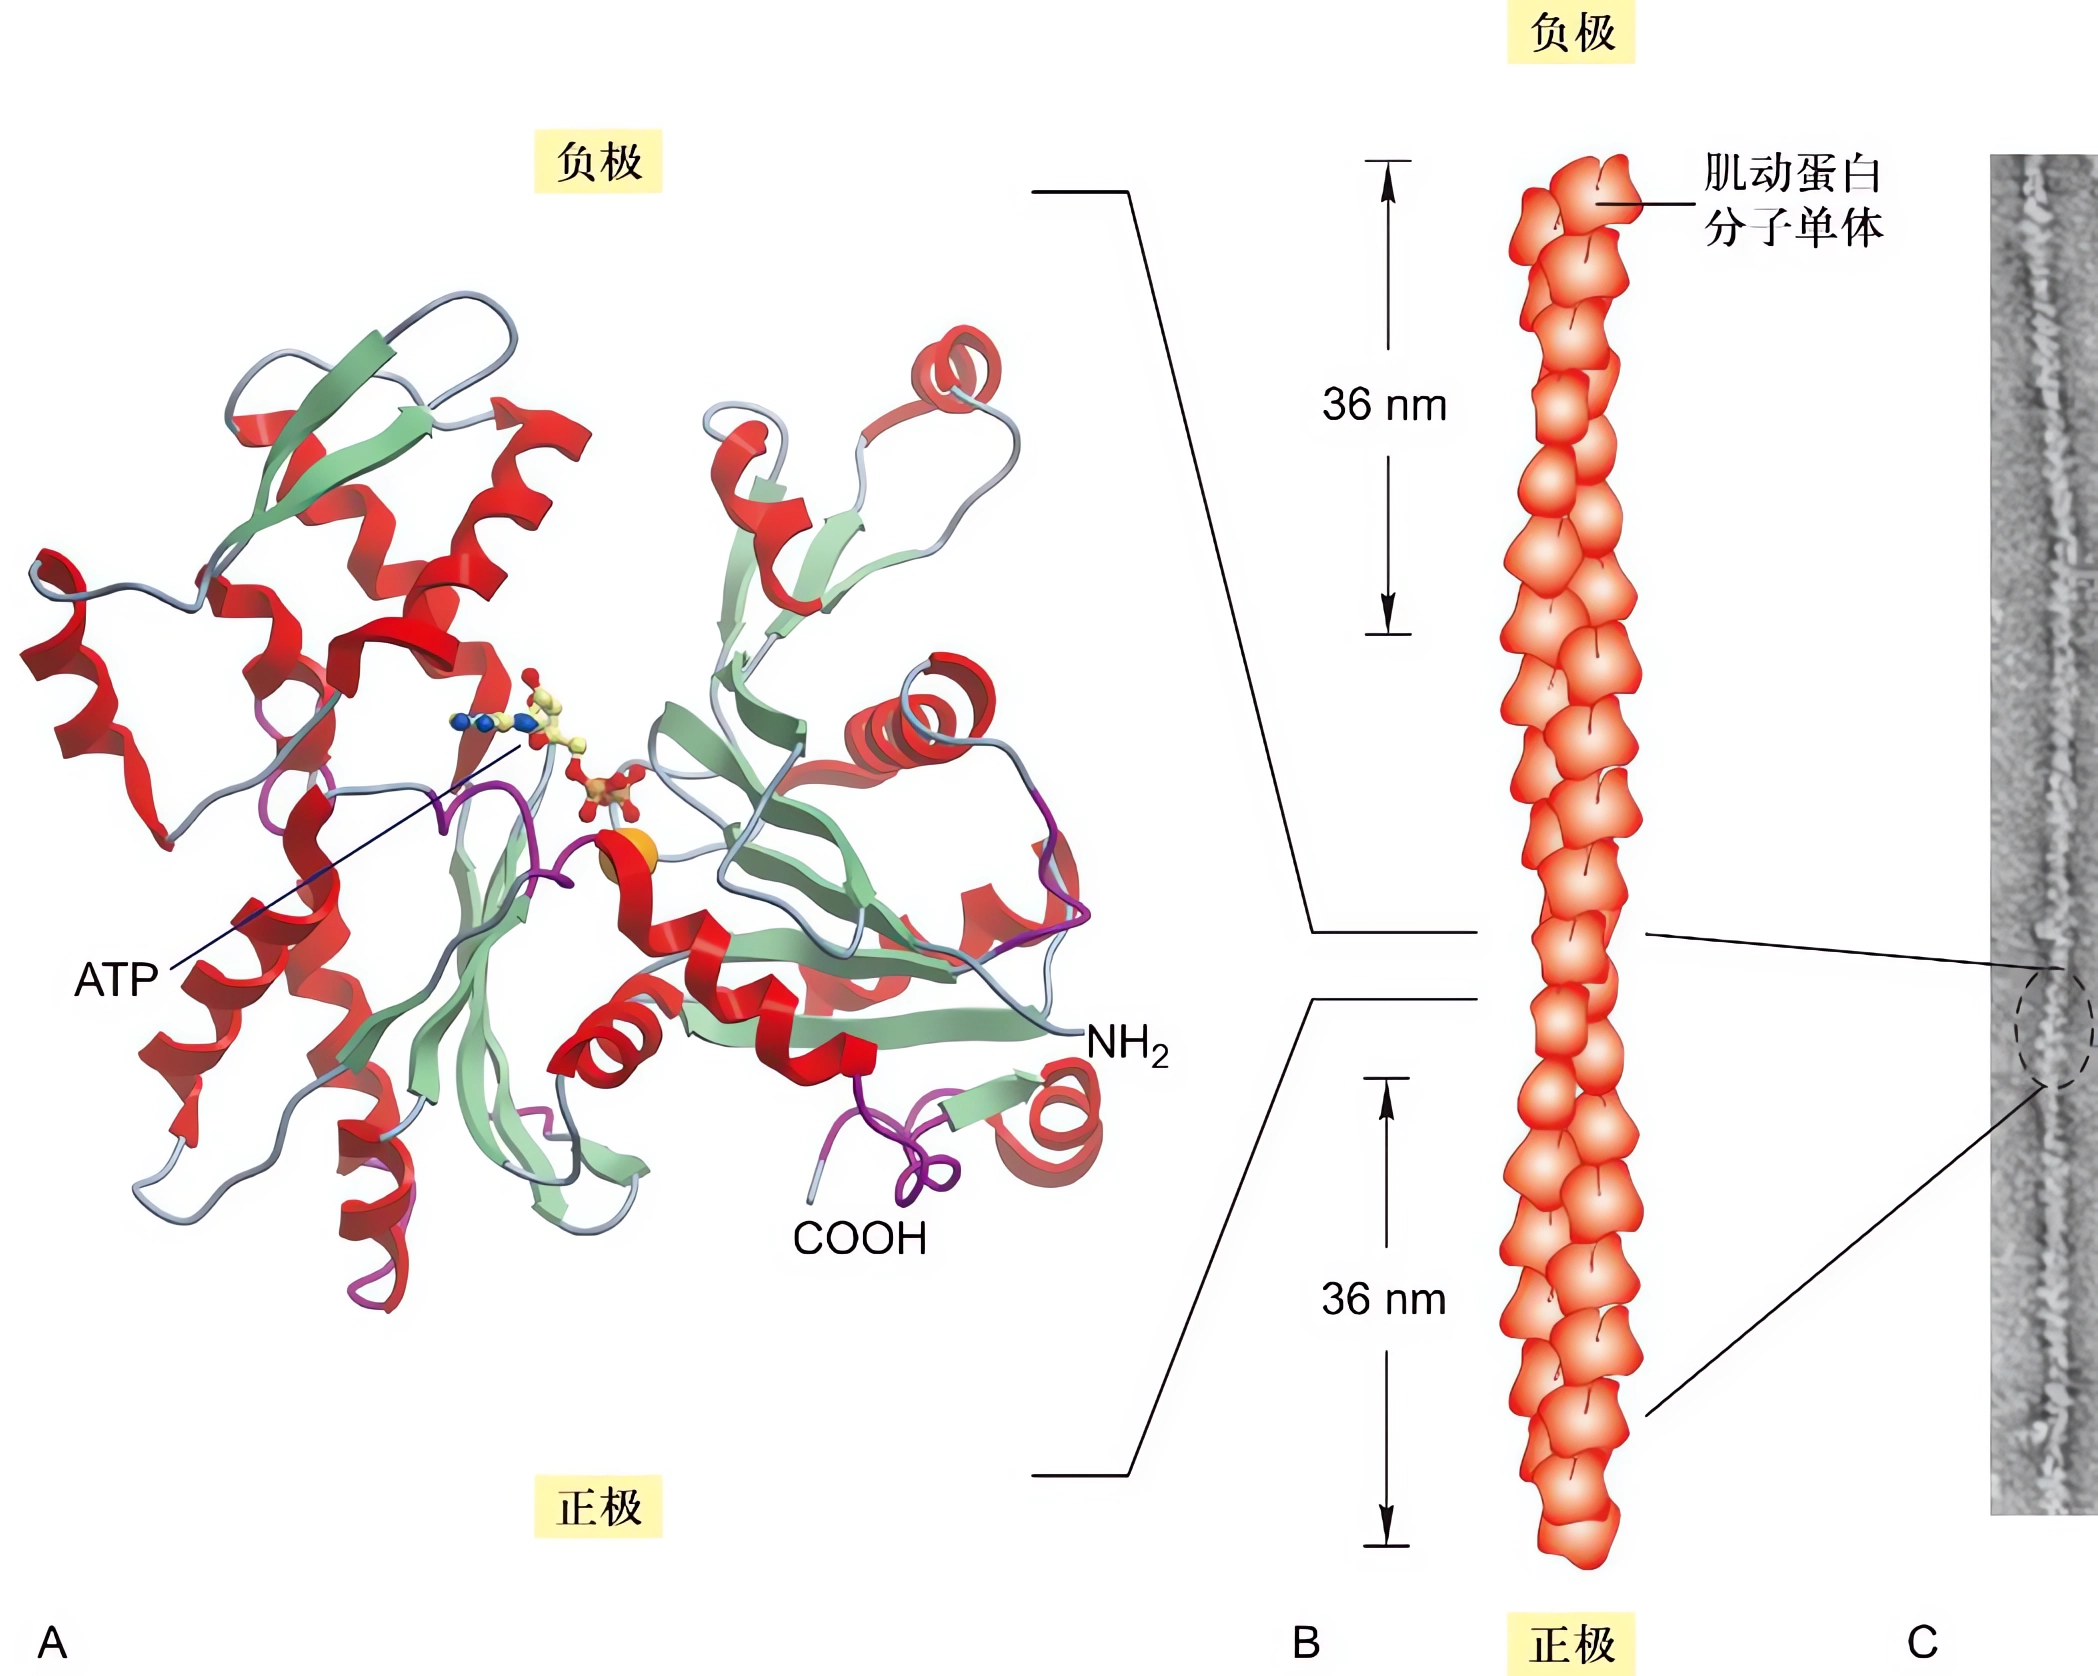
\includegraphics[width=0.7\linewidth]{Pics/肌动蛋白和微丝}
	\caption{肌动蛋白单体和微丝}
	\label{fig:actin_microfibre}
\end{figure}


\section{细胞核、染色质}

\section{核糖体}

\section{细胞信号转导}

\section{细胞周期、细胞分裂}

\section{细胞增殖调控与癌细胞}





\section{细胞分化、干细胞}

\section{细胞衰老与细胞程序性死亡}

\section{细胞的社会联系}

\subsection{细胞连接}

细胞连接是细胞之间、细胞与胞外基质相连接的结构。细胞连接包括下面三类:

\begin{description}
	\item[封闭连接] 将相邻上皮细胞的质膜紧紧地连接在一起,阻止小分子物质通过。如紧密连接。
	\item[锚定连接] 将细胞与相邻细胞或胞外基质连接。组分有胞内骨架、跨膜蛋白、胞外结构。
	\item[通信连接] 介导相邻细胞的物质转运或化学、电信号的传递。如间隙连接、化学突触、电突触(间隙连接)。
\end{description}

\subsubsection{封闭连接——以紧密连接为例}

关键结构是相邻细胞膜上跨膜蛋白形成的嵴线,
